\PassOptionsToPackage{unicode=true}{hyperref} % options for packages loaded elsewhere
\PassOptionsToPackage{hyphens}{url}
%
\documentclass[]{article}
\usepackage[labelfont=bf]{caption}
\usepackage{lmodern}
\usepackage{amssymb,amsmath}
\usepackage{ifxetex,ifluatex}
\usepackage{fixltx2e} % provides \textsubscript
\ifnum 0\ifxetex 1\fi\ifluatex 1\fi=0 % if pdftex
  \usepackage[T1]{fontenc}
  \usepackage[utf8]{inputenc}
  \usepackage{textcomp} % provides euro and other symbols
\else % if luatex or xelatex
  \usepackage{unicode-math}
  \defaultfontfeatures{Ligatures=TeX,Scale=MatchLowercase}
\fi
% use upquote if available, for straight quotes in verbatim environments
\IfFileExists{upquote.sty}{\usepackage{upquote}}{}
% use microtype if available
\IfFileExists{microtype.sty}{%
\usepackage[]{microtype}
\UseMicrotypeSet[protrusion]{basicmath} % disable protrusion for tt fonts
}{}
\IfFileExists{parskip.sty}{%
\usepackage{parskip}
}{% else
\setlength{\parindent}{0pt}
\setlength{\parskip}{6pt plus 2pt minus 1pt}
}
\usepackage{hyperref}
\usepackage{float}
\hypersetup{
            pdftitle={Informe: difracción de electrones},
            pdfauthor={Agustín Santiago Zuretti (95605); Fabrizio Sebastián Graffe (93158); Joaquin Torré Zaffaroni (98314)},
            pdfborder={0 0 0},
            breaklinks=true}
\urlstyle{same}  % don't use monospace font for urls
\usepackage{longtable,booktabs}
% Fix footnotes in tables (requires footnote package)
\IfFileExists{footnote.sty}{\usepackage{footnote}\makesavenoteenv{longtable}}{}
\usepackage{graphicx,grffile}
\makeatletter
\def\maxwidth{\ifdim\Gin@nat@width>\linewidth\linewidth\else\Gin@nat@width\fi}
\def\maxheight{\ifdim\Gin@nat@height>\textheight\textheight\else\Gin@nat@height\fi}
\makeatother
% Scale images if necessary, so that they will not overflow the page
% margins by default, and it is still possible to overwrite the defaults
% using explicit options in \includegraphics[width, height, ...]{}
\setkeys{Gin}{width=\maxwidth,height=\maxheight,keepaspectratio}
\setlength{\emergencystretch}{3em}  % prevent overfull lines
\providecommand{\tightlist}{%
  \setlength{\itemsep}{0pt}\setlength{\parskip}{0pt}}
\setcounter{secnumdepth}{0}
% Redefines (sub)paragraphs to behave more like sections
\ifx\paragraph\undefined\else
\let\oldparagraph\paragraph
\renewcommand{\paragraph}[1]{\oldparagraph{#1}\mbox{}}
\fi
\ifx\subparagraph\undefined\else
\let\oldsubparagraph\subparagraph
\renewcommand{\subparagraph}[1]{\oldsubparagraph{#1}\mbox{}}
\fi

% set default figure placement to htbp
\makeatletter
\def\fps@figure{htbp}
\makeatother


\title{Informe: difracción de electrones}
\author{Agustín Santiago Zuretti (95605) \and Fabrizio Sebastián Graffe (93158) \and Joaquin Torré Zaffaroni (98314)}
\date{}

\begin{document}
\maketitle

{
\setcounter{tocdepth}{3}
\tableofcontents
}
\newpage

\hypertarget{resumen}{%
\subsection{Resumen}\label{resumen}}

El trabajo práctico consiste en hacer pasar un haz de electrones,
acelerados por un potencial V, a través de un policristal de grafito y
observar el diagrama de interferencia que estos producen sobre una
pantalla de fósforo, pudiendo así calcular la distancia interplanar del
cristal, y la longitud de onda del haz difractado.

\hypertarget{introducciuxf3n}{%
\subsection{Introducción}\label{introducciuxf3n}}

La primera persona en proponer que la materia tiene comportamiento tanto
ondulatorio como corpuscular fue Louis de Broglie, en 1924. Así como se
sabía que la luz tiene propiedades ondulatorias y corpusculares, postuló
que la materia también tendría una dualidad en su comportamiento.

Los primeros en observar el fenómeno de difracción fueron Davisson y
Germer en los laboratorios de Bell Telephone. Ellos se encontraban
estudiando la dispersión de un haz de electrones contra un blanco de
níquel. Luego de un largo periodo de bombardeo de electrones notaron
sobre la placa receptora máximos y mínimos de intensidad, en función del
ángulo y la tensión de aceleración.

Al notar este fenómeno lo reprodujeron con diferentes monocristales
logrando deducir las longitudes de onda de manera trigonométrica,
conociendo la tensión de aceleración, la distancia interplanar del
cristal y el diámetro de proyección.

\[f = \frac{E}{h}\]

\[\lambda = \frac{h}{p}\]

Donde E y p son la energía y cantidad de movimiento del electrón
respectivamente y h la constante de Planck.

De esta manera encontraron evidencia de un comportamiento de la materia
que no corresponde al modelo de partícula sino a un modelo de onda; es
decir, la materia también presentaba una dualidad onda-partícula en su
comportamiento.

\begin{figure}[H]
\centering
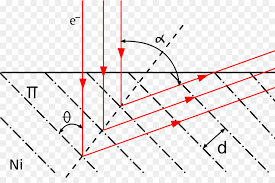
\includegraphics{difraccion.png}
\caption{Difracción de electrones.}
\end{figure}

\begin{figure}[H]
\centering
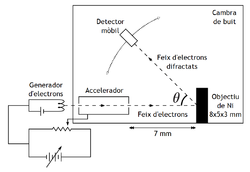
\includegraphics{experimento.png}
\caption{Dispositivo experimental de Davisson y Germer.}
\end{figure}

\newpage

\hypertarget{muxe9todo-experimental}{%
\subsection{Método experimental}\label{muxe9todo-experimental}}

\begin{figure}[H]
\centering
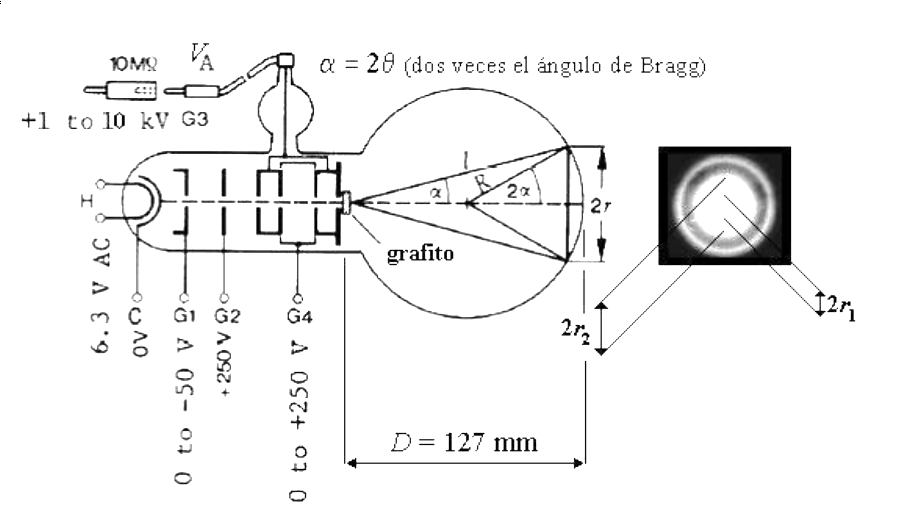
\includegraphics{geometria_experimento.png}
\caption{Dispositivo experimental}
\end{figure}

Para llevar a cabo la experiencia se utilizó un bulbo en el cual
electrones acelerados mediante un potencial atraviesan un policristal de
grafito y son difractados con cierto ángulo, finalmente chocando contra
una placa de fósforo.

Cada uno de los potenciales que se ven en la figura cumple una función.
G1 es un potencial de frenado que detiene a los electrones más débiles.
G2 y G4 enfocan y coliman el haz de electrones y G3 se encarga de
acelerarlos.

El fenómeno de difracción se manifiesta en el bulbo mediante anillos que
varían su radio dependiendo del potencial que acelera los electrones.

Las herramientas utilizadas en la experiencia fueron un multímetro para
medir el potencial de aceleración y un calibre para medir el diámetro de
los anillos de difracción.

\hypertarget{instrumentos-utilizados}{%
\subsubsection{Instrumentos utilizados}\label{instrumentos-utilizados}}

\begin{itemize}
\tightlist
\item
  Fuente de alta tensión
\item
  Tubo de difracción de electrones
\item
  Pantalla de fósforo
\item
  Cables conductores
\item
  Resistencias (10M )
\item
  Fuente VDC
\item
  Calibre
\item
  Divisor de tensión para lectura del altimetría
\item
  Altímetro
\end{itemize}

\hypertarget{procedimiento-de-mediciuxf3n}{%
\subsubsection{Procedimiento de
medición}\label{procedimiento-de-mediciuxf3n}}

\begin{enumerate}
\def\labelenumi{\arabic{enumi}.}
\tightlist
\item
  Se arma el banco de medición con los dispositivos ya nombrados como se
  ve en la figura 3. Además se usa un divisor de tensión para obtener
  una lectura más precisa.
\item
  Se va variando la tensión de la fuente y se fija.
\item
  Se miden los diámetros internos y externos de los anillos de
  Debye-Scherrer con un calibre. Se miden solo los anillos más intensos
  que se observan (para todo V).
\item
  Se repiten los pasos (2) y (3) hasta los 9kV.
\end{enumerate}

Como se ve en la figura, sobre la pantalla de fósforo se observan
anillos concéntricos denominados anillos de Debye-Scherrer. Este patrón
de interferencia se produce como ya se mencionó por la estructura del
material utilizado como red espacial de difracción, que al tener
variedad de planos con disposiciones angulares diferentes, hacen que
aparezcan circunferencias en la pantalla perpendicular a la dirección de
incidencia. En cuanto a la manera de medir los anillos, decidimos medir
su diámetro, disminuyendo el error que se cometería queriendo ubicar el
eje central de los círculos.

Al tener todas las mediciones de los anillos, podemos calcular los
ángulos de Bragg para tales. Viendo la figura, se ve claramente que se
puede determinar con la siguiente relación trigonométrica (cuya
demostración se puede ver en el apéndice)

\[\theta = \frac{1}{4} \arcsin\left (\frac{r}{R} \right )\]

Siendo \(\theta\) el ángulo de Bragg, \(r\) el diámetro del anillo y
\(R\) el diámetro del bulbo.

\hypertarget{resultados-y-anuxe1lisis}{%
\subsection{Resultados y análisis}\label{resultados-y-anuxe1lisis}}

En la siguiente tabla podemos ver los resultados obtenidos en las
mediciones. En tipo de anillo, G significa anillo grande y C anillo
chico.

\hypertarget{resultados-obtenidos}{%
\subsubsection{Resultados obtenidos}\label{resultados-obtenidos}}

En la siguiente tabla podemos ver los resultados obtenidos en las
mediciones. En la columna ``Anillo'', G significa anillo grande y C
anillo chico. Se midió el diámetro de los anillos de difracción G y C
nombrando los anillos a partir del centro de simetría mediante un
calibre (incerteza de 0,1mm):

\begin{longtable}[]{@{}llll@{}}
\toprule
\(V[K\mathrm{v}]\) & \(\Delta V[K\mathrm{v}]\) & \(d_{int}[mm]\) &
\(d_{ext}[mm]\)\tabularnewline
\midrule
\endfirsthead
\toprule
\(V[K\mathrm{v}]\) & \(\Delta V[K\mathrm{v}]\) & \(d_{int}[mm]\) &
\(d_{ext}[mm]\)\tabularnewline
\midrule
\endhead
4.07 & 0.03 & 37.1 & 43.0\tabularnewline
4.99 & 0.04 & 34.0 & 39.2\tabularnewline
6.05 & 0.05 & 31.9 & 35.5\tabularnewline
6.99 & 0.06 & 29.1 & 32.8\tabularnewline
8.04 & 0.06 & 28.7 & 31.7\tabularnewline
\bottomrule
\caption{diámetros de los anillos 1 y 2 del patrón de difracción para el
anillo mas grande.}\tabularnewline
\end{longtable}

\begin{longtable}[]{@{}llll@{}}
\toprule
\(V[K\mathrm{v}]\) & \(\Delta V[K\mathrm{v}]\) & \(d_{int}[mm]\) &
\(d_{ext}[mm]\)\tabularnewline
\midrule
\endfirsthead
\toprule
\(V[K\mathrm{v}]\) & \(\Delta V[K\mathrm{v}]\) & \(d_{int}[mm]\) &
\(d_{ext}[mm]\)\tabularnewline
\midrule
\endhead
4.07 & 0.03 & 21.1 & 25.0\tabularnewline
4.99 & 0.04 & 18.8 & 22.3\tabularnewline
6.05 & 0.05 & 17.5 & 20.0\tabularnewline
6.99 & 0.06 & 17.1 & 19.0\tabularnewline
8.04 & 0.06 & 16.4 & 18.7\tabularnewline
\bottomrule
\caption{diámetros de los anillos 1 y 2 del patrón de difracción para el
anillo mas chico.}\tabularnewline
\end{longtable}

A partir de los resultados de la medición, se prosiguió a realizar los
cálculos del ángulo de difracción según lo especificado en el apéndice
B, junto con el desarrollo de la propagación de errores. En la siguiente
sección se muestran los resultados de los cálculos.

\hypertarget{anuxe1lisis-de-los-resultados}{%
\subsubsection{Análisis de los
resultados}\label{anuxe1lisis-de-los-resultados}}

\begin{longtable}[]{@{}lll@{}}
\toprule
\(V[K\mathrm{v}]\) & \(\alpha_{int} [grad]\) &
\(\alpha_{ext} [grad]\)\tabularnewline
\midrule
\endfirsthead
\toprule
\(V[K\mathrm{v}]\) & \(\alpha_{int} [grad]\) &
\(\alpha_{ext} [grad]\)\tabularnewline
\midrule
\endhead
4.07 \(\pm\) 0.04 & 4.78 \(\pm\) 0.27 & 5.68 \(\pm\) 0.32\tabularnewline
4.99 \(\pm\) 0.04 & 4.26 \(\pm\) 0.25 & 5.06 \(\pm\) 0.29\tabularnewline
6.05 \(\pm\) 0.06 & 3.96 \(\pm\) 0.23 & 4.53 \(\pm\) 0.26\tabularnewline
6.99 \(\pm\) 0.06 & 3.87 \(\pm\) 0.23 & 3.96 \(\pm\) 0.25\tabularnewline
8.04 \(\pm\) 0.06 & 3.71 \(\pm\) 0.22 & 4.23 \(\pm\) 0.25\tabularnewline
\bottomrule
\caption{ángulo de Bragg para anillo mas grande.}\tabularnewline
\end{longtable}

\begin{longtable}[]{@{}lll@{}}
\toprule
\(V[K\mathrm{v}]\) & \(\alpha_{int} [grad]\) &
\(\alpha_{ext} [grad]\)\tabularnewline
\midrule
\endfirsthead
\toprule
\(V[K\mathrm{v}]\) & \(\alpha_{int} [grad]\) &
\(\alpha_{ext} [grad]\)\tabularnewline
\midrule
\endhead
4.07 \(\pm\) 0.03 & 4.78 \(\pm\) 0.27 & 9.90 \(\pm\) 0.32\tabularnewline
4.99 \(\pm\) 0.04 & 4.26 \(\pm\) 0.25 & 5.06 \(\pm\) 0.29\tabularnewline
6.05 \(\pm\) 0.05 & 3.96 \(\pm\) 0.23 & 4.53 \(\pm\) 0.26\tabularnewline
6.99 \(\pm\) 0.06 & 3.87 \(\pm\) 0.23 & 3.96 \(\pm\) 0.25\tabularnewline
8.04 \(\pm\) 0.06 & 3.71 \(\pm\) 0.22 & 4.23 \(\pm\) 0.25\tabularnewline
\bottomrule
\caption{ángulo de Bragg para anillo mas chico.}\tabularnewline
\end{longtable}

Dado que en la naturaleza el fenómeno se presenta de manera continua,
los electrones difractados tienen su ángulo de difracción definido por
una distribución de probabilidad y por lo tanto las observaciones que
proporcionen el menor error experimental serán las mediciones de los
diámetros internos y externos de los anillos. Es por ello que los
ángulos se presentan para un sub-índice interno o externo.

Observando la tabla 2, se ve claramente que el ángulo de difracción
disminuye con el aumento de la tensión. Es de destacar que para este
experimento únicamente se tomó las mediciones de los diámetros de los
primeros 2 anillos (empezando desde el centro), dado que la intensidad
del siguiente anillo ya era muy baja. Al aumentar la tensión, la
intensidad del tercer anillo aumentaba y por supuesto su ángulo de
difracción también disminuye.

También obtuvimos la longitud de onda de los electrones según la tensión
aplicada. (ver anexo B)

\begin{longtable}[]{@{}llll@{}}
\toprule
\(V[K\mathrm{v}]\) & \(\Delta V [K\mathrm{v}]\) & \(\lambda [\AA]\) &
\(\Delta \lambda [\AA]\)\tabularnewline
\midrule
\endfirsthead
\toprule
\(V[K\mathrm{v}]\) & \(\Delta V [K\mathrm{v}]\) & \(\lambda [\AA]\) &
\(\Delta \lambda [\AA]\)\tabularnewline
\midrule
\endhead
4.07 & 0.03 & 0.1918585131 &\tabularnewline
4.99 & 0.04 & 0.1731942208 &\tabularnewline
6.05 & 0.05 & 0.1572106535 &\tabularnewline
6.99 & 0.06 & 0.1461916664 &\tabularnewline
8.04 & 0.06 & 0.1362422209 &\tabularnewline
\bottomrule
\caption{longitudes de onda (aplicando corrección
relativista)}\tabularnewline
\end{longtable}

La energía del electrón es la misma que la del campo eléctrico en la que
se encuentra y que va a recorrer, por lo tanto tiene sentido que al
incrementar la energía del electrón, disminuye su longitud de onda. Las
ondas más energéticas son aquellas de corta longitud de onda y gran
frecuencia.

\begin{longtable}[]{@{}llllll@{}}
\toprule
\begin{minipage}[b]{0.12\columnwidth}\raggedright
\(V[K\mathrm{v}]\)\strut
\end{minipage} & \begin{minipage}[b]{0.16\columnwidth}\raggedright
\(\Delta V [K\mathrm{v}]\)\strut
\end{minipage} & \begin{minipage}[b]{0.21\columnwidth}\raggedright
\(\lambda_{relativista} [\AA]\)\strut
\end{minipage} & \begin{minipage}[b]{0.14\columnwidth}\raggedright
\(\lambda_{clasico} [\AA]\)\strut
\end{minipage} & \begin{minipage}[b]{0.13\columnwidth}\raggedright
\(\Delta \lambda [\AA]\)\strut
\end{minipage} & \begin{minipage}[b]{0.08\columnwidth}\raggedright
\(\varepsilon\) \%\strut
\end{minipage}\tabularnewline
\midrule
\endfirsthead
\toprule
\begin{minipage}[b]{0.12\columnwidth}\raggedright
\(V[K\mathrm{v}]\)\strut
\end{minipage} & \begin{minipage}[b]{0.16\columnwidth}\raggedright
\(\Delta V [K\mathrm{v}]\)\strut
\end{minipage} & \begin{minipage}[b]{0.21\columnwidth}\raggedright
\(\lambda_{relativista} [\AA]\)\strut
\end{minipage} & \begin{minipage}[b]{0.14\columnwidth}\raggedright
\(\lambda_{clasico} [\AA]\)\strut
\end{minipage} & \begin{minipage}[b]{0.13\columnwidth}\raggedright
\(\Delta \lambda [\AA]\)\strut
\end{minipage} & \begin{minipage}[b]{0.08\columnwidth}\raggedright
\(\varepsilon\) \%\strut
\end{minipage}\tabularnewline
\midrule
\endhead
\begin{minipage}[t]{0.12\columnwidth}\raggedright
4.07\strut
\end{minipage} & \begin{minipage}[t]{0.16\columnwidth}\raggedright
0.03\strut
\end{minipage} & \begin{minipage}[t]{0.21\columnwidth}\raggedright
0.1918585\strut
\end{minipage} & \begin{minipage}[t]{0.14\columnwidth}\raggedright
0.1922402\strut
\end{minipage} & \begin{minipage}[t]{0.13\columnwidth}\raggedright
0.000382\strut
\end{minipage} & \begin{minipage}[t]{0.08\columnwidth}\raggedright
0.20\strut
\end{minipage}\tabularnewline
\begin{minipage}[t]{0.12\columnwidth}\raggedright
4.99\strut
\end{minipage} & \begin{minipage}[t]{0.16\columnwidth}\raggedright
0.04\strut
\end{minipage} & \begin{minipage}[t]{0.21\columnwidth}\raggedright
0.1731942\strut
\end{minipage} & \begin{minipage}[t]{0.14\columnwidth}\raggedright
0.1736165\strut
\end{minipage} & \begin{minipage}[t]{0.13\columnwidth}\raggedright
0.000422\strut
\end{minipage} & \begin{minipage}[t]{0.08\columnwidth}\raggedright
0.24\strut
\end{minipage}\tabularnewline
\begin{minipage}[t]{0.12\columnwidth}\raggedright
6.05\strut
\end{minipage} & \begin{minipage}[t]{0.16\columnwidth}\raggedright
0.05\strut
\end{minipage} & \begin{minipage}[t]{0.21\columnwidth}\raggedright
0.1572107\strut
\end{minipage} & \begin{minipage}[t]{0.14\columnwidth}\raggedright
0.1576753\strut
\end{minipage} & \begin{minipage}[t]{0.13\columnwidth}\raggedright
0.000465\strut
\end{minipage} & \begin{minipage}[t]{0.08\columnwidth}\raggedright
0.30\strut
\end{minipage}\tabularnewline
\begin{minipage}[t]{0.12\columnwidth}\raggedright
6.99\strut
\end{minipage} & \begin{minipage}[t]{0.16\columnwidth}\raggedright
0.06\strut
\end{minipage} & \begin{minipage}[t]{0.21\columnwidth}\raggedright
0.1461917\strut
\end{minipage} & \begin{minipage}[t]{0.14\columnwidth}\raggedright
0.1466907\strut
\end{minipage} & \begin{minipage}[t]{0.13\columnwidth}\raggedright
0.000499\strut
\end{minipage} & \begin{minipage}[t]{0.08\columnwidth}\raggedright
0.34\strut
\end{minipage}\tabularnewline
\begin{minipage}[t]{0.12\columnwidth}\raggedright
8.04\strut
\end{minipage} & \begin{minipage}[t]{0.16\columnwidth}\raggedright
0.06\strut
\end{minipage} & \begin{minipage}[t]{0.21\columnwidth}\raggedright
0.1362422\strut
\end{minipage} & \begin{minipage}[t]{0.14\columnwidth}\raggedright
0.1367771\strut
\end{minipage} & \begin{minipage}[t]{0.13\columnwidth}\raggedright
0.000535\strut
\end{minipage} & \begin{minipage}[t]{0.08\columnwidth}\raggedright
0.39\strut
\end{minipage}\tabularnewline
\bottomrule
\caption{longitudes de onda y sus errores calculados para cada
tensión.}\tabularnewline
\end{longtable}

Y lógicamente, a medida que los electrones van ganando energía cinética
el error relativo por no usar la corrección relativista se hace más
relevante.

Luego, determinamos qué familias de planos contribuyen a la formación de
los anillos observados, usando la simulación del punto h del
cuestionario. Para facilitar el análisis de los datos, graficamos los
anillos calculados y los medidos en función de las distintas tensiones
aplicadas.

El primer anillo (empezando desde el centro) corresponde a la distancia
interplanar del cristal con distancia de \(2,1386 \AA\).

\begin{longtable}[]{@{}lll@{}}
\toprule
\(Diametro[mm]\) & \(d=2.1386 \AA, n=1\) & \(\varepsilon\)
\%\tabularnewline
\midrule
\endfirsthead
\toprule
\(Diametro[mm]\) & \(d=2.1386 \AA, n=1\) & \(\varepsilon\)
\%\tabularnewline
\midrule
\endhead
21.1 \(\pm\) 0.1 & 22.8 & 7.5\tabularnewline
18.8 \(\pm\) 0.1 & 20.4 & 7.8\tabularnewline
17.5 \(\pm\) 0.1 & 18.6 & 5.9\tabularnewline
17.1 \(\pm\) 0.1 & 17.3 & 1.1\tabularnewline
16.4 \(\pm\) 0.1 & 16.2 & 1.2\tabularnewline
\bottomrule
\caption{comparación de diámetros internos obtenidos experimentalmente
con diámetro para n=1 y distancia interplanar 2,1386 Å}\tabularnewline
\end{longtable}

El segundo anillo corresponde a la distancia \(1,2340 \AA\).

\begin{longtable}[]{@{}lll@{}}
\toprule
\(Diametro[mm]\) & \(d=1.2340 \AA, n=1\) & \(\varepsilon\)
\%\tabularnewline
\midrule
\endfirsthead
\toprule
\(Diametro[mm]\) & \(d=1.2340 \AA, n=1\) & \(\varepsilon\)
\%\tabularnewline
\midrule
\endhead
37.1 \(\pm\) 0.1 & 39.2 & 5.3\tabularnewline
34.0 \(\pm\) 0.1 & 35.2 & 3.4\tabularnewline
31.9 \(\pm\) 0.1 & 32.2 & 0.9\tabularnewline
29.1 \(\pm\) 0.1 & 29.8 & 2.3\tabularnewline
28.7 \(\pm\) 0.1 & 27.9 & 2.7\tabularnewline
\bottomrule
\caption{comparación de diámetros externos obtenidos experimentalmente
con diámetro para n=1 y distancia interplanar 1,2340 \AA}\tabularnewline
\end{longtable}

\begin{figure}[H]
\centering
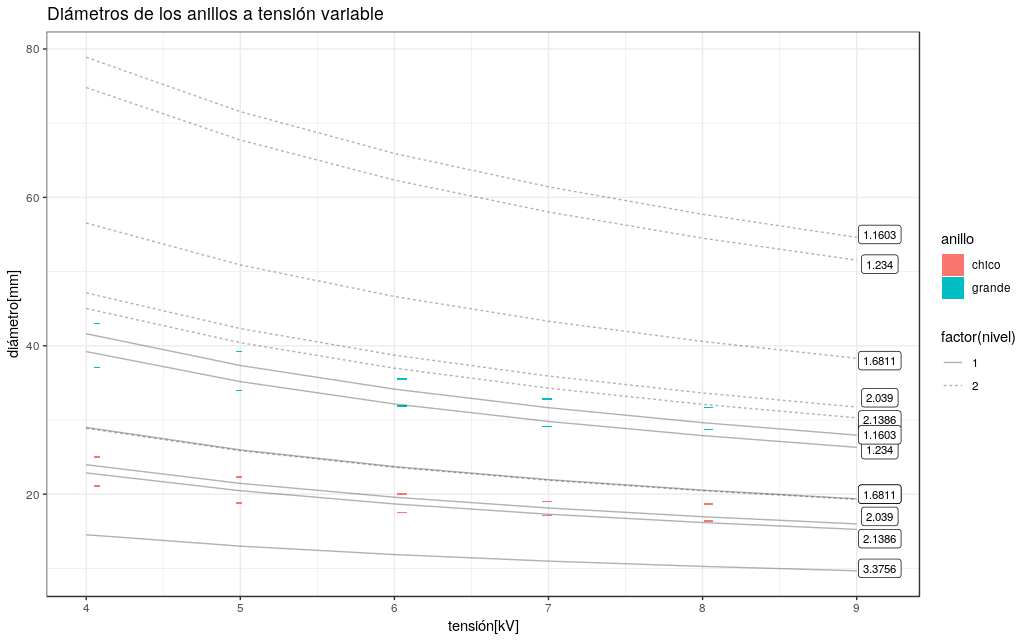
\includegraphics{resultados_experimentales.png}
\caption{Resultados experimentales.}
\end{figure}

En la figura 4 superponemos los resultados experimentales y los valores
de los diámetros en función de la tensión para algunas distancias
interplanares conocidas.\\
A partir del gráfico de los resultados podemos ver que los anillos
medidos (que, a diferencia de las líneas que representan los anillos
teóricos calculados antes, \emph{sí} tienen espesor) encierran en su
parte brillante a más de una curva de distancia interplanar.

En el caso del anillo grande, vemos que se encierra al anillo de orden
de difracción \(1\) del plano con \(d = 1.16\AA\) y del mismo orden de
difracción \(d = 1.2340\AA\). En el chico, vemos que los anillos
encerrados son \(d = 2.0390\AA\) y \(d = 2.1386\) del orden de
difracción \(1\).

Postulamos, entonces, que no sólo una distancia interplanar contribuye
al patrón de interferencia que observamos con los anillos, sino que son
múltiples.

Estas observaciones se cumplen para todas las mediciones excepto la de
\(\mathrm{V} = (8.04 \pm 0.06)K\mathrm{v}\), en la que en ambos anillos
sólo queda una distancia interplanar adentro. En ambos casos hay un
aumento del valor que logra esto. Esto puede ser una sobre-estimación
del valor, y puede deberse a un error bajo en la medición del diámetro.
Para definirlo, sólo tomamos el error de apreciación del instrumento
(\(e_{ap} = 0.1mm\)), pero las condiciones de medición aumentan el
error: el hecho de que se mida el punto en el que la luz deja de ser
brillante y que no sea una línea tan definida, la medición en la
oscuridad, la curvatura del bulbo.

Teniendo en cuenta estos factores que aumentan el error, podríamos tomar
el hecho de que en la última medición se descarte una distancia
interplanar en cada anillo es debdio a una sub-estimación del error.
Esto cobra especial importancia en el caso del anillo chico, donde se ve
que la diferencia es mínima.

\hypertarget{conclusiones}{%
\subsection{Conclusiones}\label{conclusiones}}

Los resultados obtenidos satisfacen la hipótesis de que la materia
corpuscular también presenta cualidades ondulatorias. Las longitudes de
onda para los electrones coinciden mayormente con lo calculado teóricamente en
función de las tensiones medidas. El máximo error relativo fue del
7.8\%, un número tal vez no tan bajo como el que se hubiera esperado, pero 
que puede ser atribuido a errores en las mediciones de los diametros de los
anillos. Los diámetros hallados experimentalmente, se ajustan a los 
diámetros calculados analiticamente expresados en el gráfico como 
{[}1.2340E-10 m, n=1{]} y {[}2.1386E-10 m, n=1{]} los cuales corresponden 
a las las distancias interplanares 1,2340 \AA y 2,1386 \AA respectivamente, 
tal como se había hallado previamente en las tablas 5 y 6. 
A su vez, por medio del gráfico pudimos observar que los diámetros de anillos correspondientes a la distancia interplanar {[}2.1386E-10 m, n=1{]} y 
{[}2.0390E-10 m, n=1{]} quedan dentro del área dada entre los diámetros 
d1int y d1ext. Y lo mismo es observado para {[}1.2340E-10 m, n=1{]} y 
{[}1.1603E-10 m, n=1{]}, los cuales quedan entre los diametros 
d2int y d2ext. La razón de que ocurra éste fenómeno podría ser que mas de 
una distancia interplanar esté contribuyendo a la formación de los 
anillos (en este caso son 2 distancias interplanares distintas para cada 
anillo, d1 y d2).

\newpage

\hypertarget{apuxe9ndice-a---cuestionario}{%
\subsection{Apéndice A -
cuestionario}\label{apuxe9ndice-a---cuestionario}}

\hypertarget{experimento-de-davison-germer-y-la-ley-de-bragg}{%
\subsubsection{Experimento de Davison-Germer y la Ley de
Bragg}\label{experimento-de-davison-germer-y-la-ley-de-bragg}}

El experimento de Davisson y Germer demostró que los objetos
corpusculares presentaban un carácter ondulatorio, corroborando la
hipótesis de Louis-Victor de Broglie, en la que expone que toda la
materia, (electrones, átomos o moléculas), presenta características
tanto corpusculares como ondulatorias.

En este experimento, un monocristal es bombardeado con electrones
acelerados por un potencial eléctrico V. Suponiendo que los electrones
presentan un comportamiento ondulatorio, la onda incidente se refleja en
cada uno de los planos atómicos, existiendo una interferencia
constructiva de las ondas reflejadas en planos paralelos consecutivos
descritos por la Ley de Bragg.

Lo que se observa es que estos son reflejados mayoritariamente en
aquellas direcciones privilegiadas para las que exista interferencia
constructiva, lo cual demuestra la hipótesis de de broglie.

Cuando los rayos X alcanzan un átomo interactúan con sus electrones
exteriores. Estos reemiten la radiación electromagnética incidente en
diferentes direcciones y con la misma frecuencia (en realidad debido a
varios efectos hay pequeños cambios en su frecuencia). Este fenómeno se
conoce como dispersión de Rayleigh (o dispersión elástica). Los rayos X
reemitidos desde átomos cercanos interfieren entre sí constructiva o
destructivamente. Este es el fenómeno de la difracción.

\begin{figure}[H]
\centering
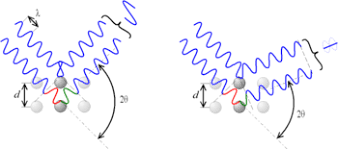
\includegraphics{bragg.png}
\caption{ley de bragg.}
\end{figure}

La radiación incidente llega a átomos consecutivos con un ligero desfase
(izquierda). La radiación dispersada por los átomos (círculos azules)
interfiere con radiación dispersada por átomos adyacentes. Las
direcciones en las que los círculos se superponen son direcciones de
interferencia constructiva.

La interferencia es constructiva cuando la diferencia de fase entre la
radiación emitida por diferentes átomos es proporcional a 2 pi. Esta
condición se expresa en la ley de Bragg:

\[\ n \lambda = 2 d \sin(\theta)\]

\hypertarget{relaciuxf3n-entre-longitud-de-onda-y-energuxeda-cinuxe9tica}{%
\subsubsection{Relación entre longitud de onda y energía
cinética}\label{relaciuxf3n-entre-longitud-de-onda-y-energuxeda-cinuxe9tica}}

La ecuación que nos va a permitir relacionar la longitud de onda y la
energía cinética principalmente será la de de Broglie:
\(\lambda = \frac{h}{p}\), y dependiendo de las condiciones del
problema, podemos usar la ecuación de la energía cinética de la mecánica
clásica o deberemos usar la de la mecánica relativista.

En el caso clásico, donde la energía cinética del electrón es
relativamente pequeña respecto a la energía asociada a la masa en
reposo, podemos usar la asociación entre energía cinética y cantidad de
movimiento lineal:

\[\ n \lambda = \frac{h}{\sqrt{2m_e 10keV}} = 0,1226 \AA\]

\[\mathrm{E}_c = \frac{p^2}{2m}\]

Al reemplazar la cantidad de movimiento \(p\) por \(\frac{h}{p}\)
obtenemos:

\[ \lambda = \frac{h}{\sqrt{2m\mathrm{E}_c}} \]

En el caso que la aproximación clásica no se pueda utilizar dadas las
condiciones del problema, será necesario usar las ecuaciones de la
mecánica relativista. En este caso tenemos el par de ecuaciones:

\[
\left\{\begin{matrix}
    \mathrm{E} = mc^2 + \mathrm{E}_c + \mathrm{E}_p\\
    \mathrm{E}^2 = (pc)^2 + (mc^2)^2
\end{matrix}\right.
\]

Para este experimento, nos interesa analizar el estado del electrón en
el instante que sale del tubo. Si definimos el potencial eléctrico en
ese punto como el cero de referencia podemos considerar
\(\mathrm{E}_p = 0\). En el viaje desde la expulsión desde el electrón
hasta el choque contra la pantalla de fósforo no hay es necesario
considerar ningún campo eléctrico o gravitatorio.

Sustituyendo la primera ecuación en la segunda, y aplicando la misma
sustitución de cantidad de movimiento por las variables asociadas a la
onda de la materia, terminamos con la siguiente expresión:

\[\lambda = \frac{hc}{\sqrt{\mathrm{E}_c(\mathrm{E}_c + 2mc^2)}}\]

\hypertarget{cambio-de-la-longitud-de-onda-de-los-electrones}{%
\subsubsection{Cambio de la longitud de onda de los
electrones}\label{cambio-de-la-longitud-de-onda-de-los-electrones}}

Como \(\lambda = \frac{h}{p}\) (de los postulados de de Broglie), se
debe campiar el impulso de los electrones para cambiar su onda. Esto lo
podemos lograr controlando la tensión del circuito acelerador.

Si \(V_{max} = 10 kV\), entonces \(\mathrm{E}_c^{max} = 10 keV\).

Utilizando la hipótesis no relativista obtenemos:

\[\lambda_{clasico} = \frac{h}{\sqrt{2m_e 10keV}} = 0,1226 \AA\]

Utilizando las ecuaciones de la mecánica relativista logramos:

\[\lambda_{relativista} = \frac{hc}{\sqrt{10keV(10keV + 2m_ec^2)}}
= 0,1220 \AA\]

Lo cual nos da un error porcentual de \(e_r \approx 0,5\%\).

\hypertarget{apariciuxf3n-de-anillos-en-el-bulbo}{%
\subsubsection{Aparición de anillos en el
bulbo}\label{apariciuxf3n-de-anillos-en-el-bulbo}}

Dado que el policristal que se utiliza en el experimento fue molido, la
orientación de las estructuras regulares del cristal se vuelve
aleatoria, y esto le termina dando una simetría de revolución a la
dispersión de las ondas de los electrones.

\hypertarget{uxe1ngulo-de-dispersiuxf3n}{%
\subsubsection{Ángulo de dispersión}\label{uxe1ngulo-de-dispersiuxf3n}}

\begin{figure}[H]
\centering
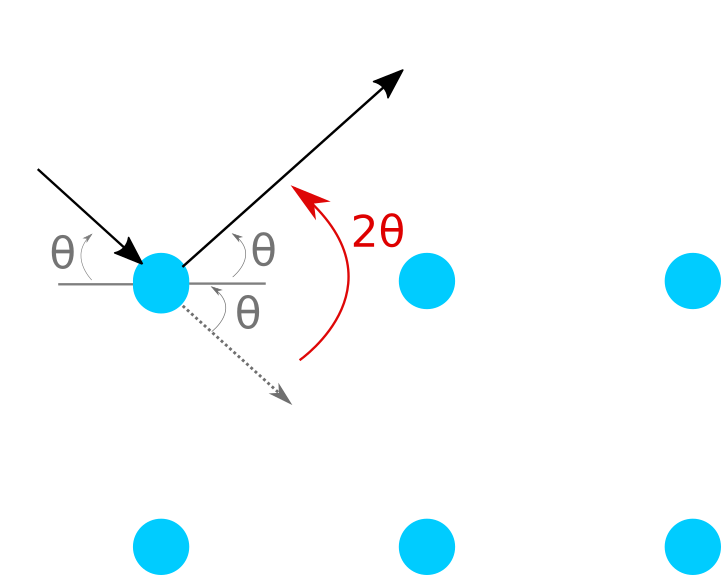
\includegraphics{cuestionario_e.svg.png}
\caption{Dispersión de las ondas bajo hipótesis de Bragg}
\end{figure}

\hypertarget{minimizaciuxf3n-del-error-de-mediciuxf3n}{%
\subsubsection{Minimización del error de
medición}\label{minimizaciuxf3n-del-error-de-mediciuxf3n}}

El calibre es un instrumento bastante sencillo con un error de
apreciación bajo (\(e_{ap} = 0.1\mathrm{mm}\)). Una opción sería medir
directamente el espesor de cada anillo, pero entonces el error de
apreciación será relativamente alto respecto al mensurando.

Una manera mejor es medir los radios internos y externos por separado,
para medir de manera indirecta el espesor. Si bien el error absoluto se
duplicará (por propagación lineal, el error de la suma es la suma de los
errores), relativamente a la magnitud que se mide será mucho menor.

\hypertarget{cuxe1lculo-del-theta-sin-aproximaciuxf3n}{%
\subsubsection{\texorpdfstring{Cálculo del \(\theta\) sin
aproximación}{Cálculo del \textbackslash{}theta sin aproximación}}\label{cuxe1lculo-del-theta-sin-aproximaciuxf3n}}

En la Figura 3 podemos ver la geometría del dispositivo experimental.
Esto nos permite ver cómo se relaciona el ángulo de dispersión (y en
definitiva el ángulo de Bragg) con las dimensiones del bulbo y de los
anillos que se observan en la pantalla de fósforo.

\begin{figure}[H]
\centering
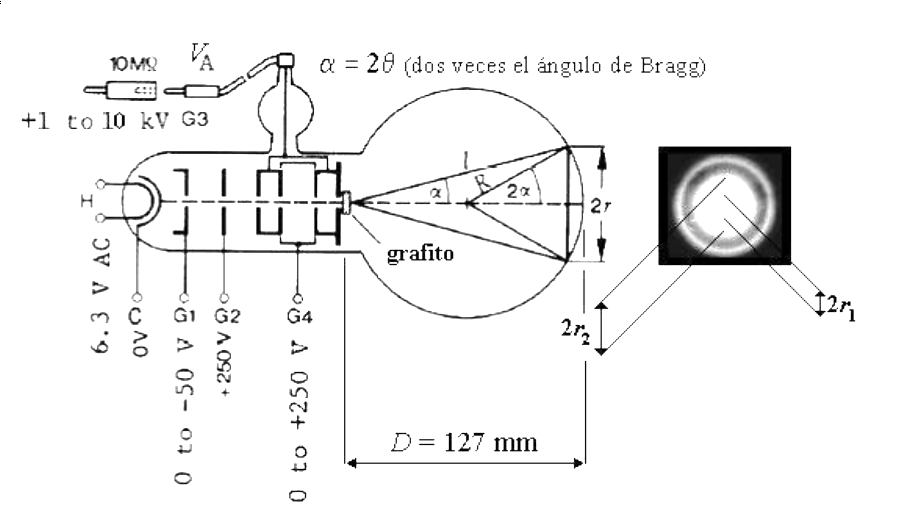
\includegraphics{geometria_experimento.png}
\caption{Geometría del experimento}
\end{figure}

Usando la notación del gráfico, observamos que:

\[\sin (2\alpha) = \frac{r}{R} \Rightarrow \theta = \frac{1}{4}
\arcsin\left (\frac{r}{R} \right )\]

Y esto nos da un método sin aproximaciones para calcular el ángulo de
Bragg, ya que \(r\) es lo que medimos (el radio del anillo) y \(R\) es
conocido (el radio del bulbo).

\hypertarget{tablas-de-theta-para-distintos-n-v-d}{%
\subsubsection{\texorpdfstring{Tablas de \(\theta\) para distintos
\(n, v, d\)}{Tablas de \textbackslash{}theta para distintos n, v, d}}\label{tablas-de-theta-para-distintos-n-v-d}}

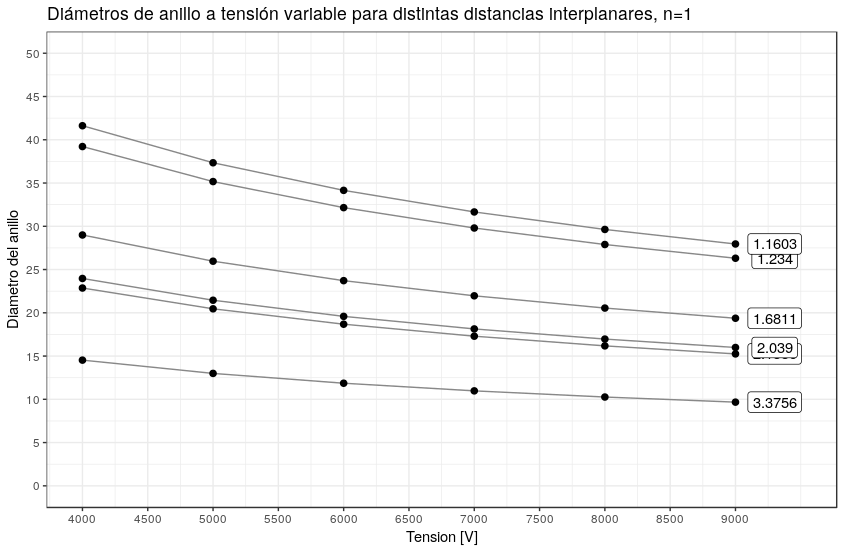
\includegraphics{nivel_1.png} 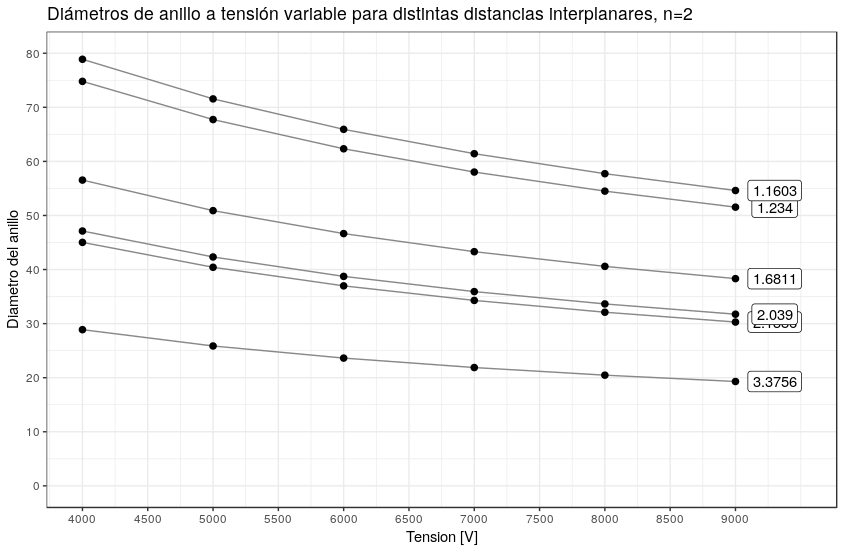
\includegraphics{nivel_2.png}

\newpage

\hypertarget{apuxe9ndice-b}{%
\subsection{Apéndice B}\label{apuxe9ndice-b}}

Utilizando los postulados de De Broglie y la hipótesis no relativista
(que en el apéndice se ve que tiene un error menor al \(1\%\) en este
orden de energías) podemos calcular las longitudes de onda de las
funciones de onda asociadas a los electrones, con la siguiente relación:
\[\lambda = \frac{h}{\sqrt{2m_e E_c}}\] donde \(h\) es la constante de
Planck, \(m_e\) la masa del electrón y \(E_c\) la energia cinetica del
electron a causa de la tensión con la cual se acelera a los electrones.

Para calcular \(\Delta \lambda\) utilizamos propagación lineal de
variables. Dado que las energias de los electrones estan en el orden de
los KeV, lo cual es mucho menor a \(m_o c^2\), podemos usar la siguiente
expresión para el calculo de la incerteza:

\[\Delta \lambda(V, \Delta V) =
\left |
    \frac{\partial}{\partial V} \left (
        \frac{h}{\sqrt{2m_e eV}}
    \right )(V) \times \Delta V
\right | = \frac{h}{\sqrt{2m_e}\ eV^{3/2}} \Delta V\]

\end{document}
